

\section{Полиномиальная регрессия}

Не все функции можно эффективно аппроксимировать линейными моделями, но многочлены справляются с этой задачей гораздо лучше. Полиномиальная регрессия является улучшением линейной модели: в ней добавляются дополнительные предикторы, представляющие собой степени исходных переменных. В этой задаче необходимо аппроксимировать функцию $y:\mathbb{R} \rightarrow \mathbb{R}$ функцией (полиномом) $a(x, \vec{\theta}) =  \sum\limits_{i=0}^n x^i \theta_{i}$. Это делается путём подбора $\theta\in\mathbb{R}^{(n+1)}$, минимизируя
$\sum\limits_{i=1}^N L(x_i,\vec{\theta})$, где $L(x,\vec{\theta})$~--- функция потерь, которая равна $|a(x,\vec{\theta})-y(x)|$, $|a(x,\vec{\theta})-y(x)|^2$ или любому другому симметричному неотрицательному функционалу, а $x_i$~--- элементы выборки размера $N$.

Возьмём функцию потерь, как в методе наименьших квадратов, выборку из $N$ элементов $\vec{x}$ и соответствующий вектор значений $\vec{y}:\, y_i = y(x_i)$.
Тогда $$\displaystyle {\begin{bmatrix}y_{1}\\y_{2}\\y_{3}\\\vdots \\y_{N}\end{bmatrix}}={\begin{bmatrix}1&x_{1}&x_{1}^{2}&\dots &x_{1}^{n}\\1&x_{2}&x_{2}^{2}&\dots &x_{2}^{n}\\1&x_{3}&x_{3}^{2}&\dots &x_{3}^{n}\\\vdots &\vdots &\vdots &\ddots &\vdots \\1&x_{N}&x_{N}^{2}&\dots &x_{N}^{n}\end{bmatrix}}{\begin{bmatrix}\theta _{0}\\\theta _{1}\\\theta _{2}\\\vdots \\\theta _{n}\end{bmatrix}}+
    \begin{bmatrix}
        \varepsilon _{0} \\\varepsilon _{1}\\\varepsilon _{2}\\\vdots \\\varepsilon _{n}
    \end{bmatrix}$$

Пусть $$X = {\begin{bmatrix}1&x_{1}&x_{1}^{2}&\dots &x_{1}^{n}\\1&x_{2}&x_{2}^{2}&\dots &x_{2}^{n}\\1&x_{3}&x_{3}^{2}&\dots &x_{3}^{n}\\\vdots &\vdots &\vdots &\ddots &\vdots \\1&x_{N}&x_{N}^{2}&\dots &x_{N}^{n}\end{bmatrix}}, \quad \vec{\varepsilon} = \begin{bmatrix}
        \varepsilon _{0} \\\varepsilon _{1}\\\varepsilon _{2}\\\vdots \\\varepsilon _{n}
    \end{bmatrix}$$.

Тогда $\vec{y}=X\vec{\theta}+\vec{\varepsilon}$. И нам нужно минимизировать $||\vec{y} - X\vec{\theta}||_2 = ||\varepsilon||_2$. По аналогичным причинам, как в методе наименьших квадратов, оптимальное значение $\theta:\ \hat{\theta} = (X^T X)^{-1} X^T \vec{y}$. Матрица $X$ имеет вид матрицы Вандермонда. Как известно, чтобы она была обратима, необходимо и достаточно, чтобы $N\geq n+1$, а все $x_i$ были различны.

Также известно, что при $N=n+1$ существует единственный многочлен степени $n$, который проходит через все $N$ точек. Он называется интерполяционным многочленом Лагранжа и имеет вид:
$$\sum\limits_{i=1}^{n+1} y_i \prod_{j\neq i}\frac{x-x_j}{x_i-x_j}$$.


К сожалению, полиномиальная регрессия также имеет немало проблем. По мере того, как мы увеличиваем сложность формулы, число признаков также увеличивается, что иногда трудно рассчитать.

Кроме того, она по своей природе нелокальна, то есть изменение значения одной точки в обучающем наборе может повлиять на подгонку полинома для точек данных, которые находятся очень далеко. Следовательно, чтобы избежать использования полинома высокой степени для всего набора данных, мы можем заменить его несколькими различными полиномиальными функциями малой степени.

\problem{Дан многочлен $f(x)$ степени $n$ и $k$ различных пар $(x, f(x))$. При каких $k$ существует бесконечного много многочленов, проходящих через все $k$ точек.}

\solution{Ответ: $0 \leq k \leq n.$

При $k \geq n+1$ существует единственный многочлен, проходящий через точки $x_1, \, x_2, \, \dots,\,x_{n+1}$. Значит, через все точки проходит не более одного многочлена.

При $k < n+1$ рассмотрим $$f(x) =A\cdot x^{n-k}\prod_{i=1}^k (x-x_i) +\sum\limits_{i=1}^k y_i \prod_{j\neq i}\frac{x-x_j}{x_i-x_j}$$
Можно взять любое $A\neq 0$. Значение в точках $x_1,\,\dots,\,x_k$ не поменяется.}

\problem{Аппроксимуруйте многочленом второй степени функцию $f(x): \ f(0)=7,\ f(1)=5,\ f(2) = 1, \ f(3)=1.$}

\solution{$$X = \begin{bmatrix}1 & 0 & 0 \\1 & 1 & 1 \\1 & 2 & 4 \\1 & 3 & 9\end{bmatrix}, \quad \vec{y} = \begin{bmatrix}
        7 \\
        5 \\
        1 \\
        1
    \end{bmatrix}$$

$$\hat{\theta} =  (X^T X)^{-1} X^T \vec{y} = \frac{1}{20}\begin{bmatrix}
        19  & -21 & 1   \\
        -21 & 49  & -15 \\
        5   & -15 & 5   \\
    \end{bmatrix}
    \begin{bmatrix}
        1 & 1 & 1 & 1 \\
        0 & 1 & 2 & 3 \\
        0 & 1 & 4 & 9
    \end{bmatrix}
    \begin{bmatrix}
        7 \\
        5 \\
        1 \\
        1
    \end{bmatrix} = \frac{1}{10}
    \begin{bmatrix}
        73  \\
        -37 \\
        5
    \end{bmatrix}
$$

То есть $\hat{y}(x) = \frac{1}{10} (5x^2 -37x+73).$

\begin{figure}[h]
    \centering
    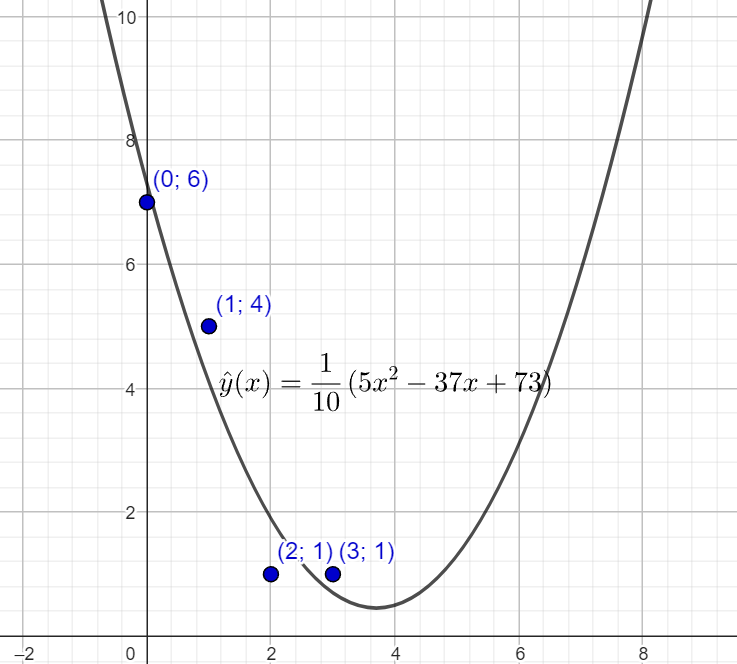
\includegraphics[width=0.5\linewidth]{chapters/nonlinear/sol_pol_1.png}
\end{figure}

\section{Сплайн-регрессия}

Чтобы преодолеть недостатки полиномиальной регрессии, мы можем использовать улучшенный метод регрессии, который вместо построения одной модели для всего набора данных делит набор данных на несколько блоков и подгоняет каждый блок отдельной моделью. Такая техника называется сплайн-регрессией. В этом случае имеется возможность осуществить регрессию сшивкой отрезков (точнее говоря, участков, т. к. они криволинейной формы) нескольких полиномов. Регрессия одним полиномом эффективна, когда множество точек выглядит приблизительно как полином, а регрессия отрезками полиномов оказывается полезной в противоположном случае, например, для функции синуса.

Точки, где происходит разделение, называются узлами. Функции, которые мы можем использовать для моделирования каждого куска/бина, называются кусочными функциями. Существуют различные кусочные функции, которые мы можем использовать для подгонки этих отдельных участков.

Пусть мы разбили $\mathbb{R}$ на $n$ частей, то есть $-\infty=x_0, \,x_1, \, \dots,\, x_{n},\,x_{n+1}=+\infty$. В узлах функции на соседних отрезках могут давать разные значения. Мы либо можем выкалывать узлы и соединять функции на полуинтервалах, тогда $$f(x) = \sum\limits_{i=0}^{n} f_i(x)\mathbb{I}[x_i;\, x_{i+1})$$

Если же мы хотим непрерывности нашей аппроксимирующей функции, то можно соединять функции на отрезках $[x_i+\varepsilon; \, x_{i+1}-\varepsilon]$ при малом $\varepsilon>0$, и затем соединять пары точек вида $(x_i-\varepsilon,\, f_{i-1}(x_i-\varepsilon))$ и $(x_i+\varepsilon,\, f_{i}(x_i+\varepsilon))$ отрезками при $i=\overline{1,n}$.

Когда мы подгоняем сплайн, где мы должны разместить узлы? Одним из потенциальных мест может быть область высокой изменчивости, потому что в этих областях коэффициенты полинома могут быстро меняться. Следовательно, одним из вариантов является размещение большего количества узлов в тех местах, где, по нашему мнению, функция может изменяться наиболее быстро, и размещение меньшего количества узлов в тех местах, где она кажется более стабильной.

Хотя эта опция может работать хорошо, на практике обычно принято размещать узлы равномерно. Один из способов сделать это - указать желаемые степени свободы, а затем заставить программное обеспечение автоматически размещать соответствующее количество узлов в одинаковых квантилях данных.

Другой вариант - опробовать разное количество узлов и посмотреть, какой вариант дает наилучшую кривую.

Более объективный подход заключается в использовании кросс-валидации. С помощью этого метода: мы удаляем часть данных, подгоняем сплайн с определенным количеством узлов к оставшимся данным, а затем используем сплайн, чтобы сделать прогноз для удаленной части данных.

Мы повторяем этот процесс несколько раз, пока каждое наблюдение не будет пропущено хотя один раз, а затем вычисляем общее перекрестное значение RMSE. Эту процедуру можно повторить для разного количества K узлов. Затем выбирается значение K, дающее наименьшее RMSE (среднеквадратическая ошибка).

Сплайновая регрессия часто дает лучшие результаты, чем полиномиальная регрессия. Это связано с тем, что в отличие от полиномов высоких степеней, которые необходимо использовать для получения гибкой подгонки, сплайны обеспечивают гибкость, увеличивая количество узлов, но сохраняя фиксированную степень.


\problem Рассмотрим задачу аппроксимации функции с помощью сплайн-регрессии. Пусть у нас есть набор данных, представляющий собой значения функции \(f(x)\) в определенных точках:

\begin{align*}
    x_0 & = 0, \quad f(x_0) = 1 \\
    x_1 & = 1, \quad f(x_1) = 2 \\
    x_2 & = 2, \quad f(x_2) = 0 \\
    x_3 & = 3, \quad f(x_3) = 3 \\
    x_4 & = 4, \quad f(x_4) = 2
\end{align*}

Постройте функции кусковой линейной регрессии (линейные сплайны) на отрезках \([x_0, x_1]\), \([x_1, x_2]\), \([x_2, x_3]\) и \([x_3, x_4]\) и соедините их в одну непрерывную функцию.

\solution
1. Отрезок \([x_0, x_1]\):\\
Два известных значения: \(f(0) = 1\) и \(f(1) = 2\). Угловой коэффициент:
$\displaystyle     a_0 = \frac{f(1) - f(0)}{x_1 - x_0} = \frac{2 - 1}{1 - 0} = 1.$ Тогда $y_0 = 1 \cdot x + 1 = x + 1.$\\
2. Отрезок \([x_1, x_2]\):\\
$\displaystyle     a_1 = \frac{f(2) - f(1)}{x_2 - x_1} = \frac{0 - 2}{2 - 1} = -2.$ Тогда $y_0 = -2 x + 4 = -2x + 4.$\\
3. Отрезок \([x_2, x_3]\):\\
$\displaystyle     a_2 = \frac{f(3) - f(2)}{x_3 - x_2} = \frac{3 - 0}{3 - 2} = 3.$ Тогда $y_0 = 3x - 6 = 3x-6.$\\
4. Отрезок \([x_3, x_4]\):
$\displaystyle     a_3 = \frac{f(4) - f(3)}{x_4 - x_3} = \frac{2 - 3}{4 - 3} = -1.$ Тогда $y_0 = -1\cdot x + 6 = -x + 6.$

Наконец, мы можем пострить нашу итоговую функцию (сплайн-регрессию):
\[
    \hat{f}(x) =
    \begin{cases}
        x + 1,   & x \in [0, 1] \\
        -2x + 4, & x \in [1, 2] \\
        3x - 6,  & x \in [2, 3] \\
        -x + 6,  & x \in [3, 4]
    \end{cases}
\]






\section*{Методы Ньютона-Рафсона, Ньютона-Гаусса}

Мы уже познакомились с задачами линейной регрессии и обсудили несколько методов их решения. Но что делать если задача нелинейна? Оказывается, что идея локальной линейности гладкой функций позволяет свести задачу к более простому. На этой идее основаны методы второго порядка - Ньютона-Рафсона и Ньютона-Гаусса.

\subsection*{Метод Ньютона-Рафсона}

Начнем немного сдалека, а именно рассмотрим задачу поиска нуля $a$ функций $f(x)$. Пусть мы находимся в точке $a^{0}$ и хотим найти такое приращение $h$, чтобы приблизиться к точке $a$: $a^{0} + h \approx a$. Применим разложение в ряд:

\begin{gather*}
    f(a^{0} + h) = f(a^{0}) + f'(a^{0})h + o(h)\\[1em]
    f(a^{0} + h) \approx f(a) = 0 \Rightarrow f(a^{0}) + f'(a^{0})h \approx 0
\end{gather*}

Откуда

\[
    h \approx - \frac{f(a^{0})}{f'(a^{0})}
\]

Значит, для поиска нуля выпуклой функций \( f \) можно применить следующий итеративный метод:

\[
    a^{k + 1} = a^{k} - \frac{f(a^{k})}{f'(a^k)}
\]

Вернемся к начальной задаче:

\begin{itemize}
    \item обучающая выборка \( X^{l} = (x_{i}, y_{i}) \), где \( x_{i} \) - вектор признаков \( i \)-го объекта
    \item \( y_{i} = y(x_{i}),\quad y: X \to Y \) - неизвестная регрессионная зависимость
    \item \( f(x, \alpha) \) - нелинейная модель регрессии, где \( \alpha \) - вектор параметров
\end{itemize}

Хотим решить задачу оптимизации методом наименьших квадратов:

\[
    Q(\alpha, X^{l}) = \sum\limits_{i = 1}^{l}\left(f(x_{i}, \alpha) - y_{i} \right)^{2} \to \min_{\alpha}
\]

Функция потерь \( Q(\alpha, X^{l}) \) выпукла и гладкая в предположений гладкости \( f(\alpha, x) \), поэтому для ее минимизаций достаточно найти нуль производной (градиента). Применяя рассуждения выше и опустив технические детали, получим следующий итерационный процесс:

\[
    \alpha^{k + 1} = \alpha^{k} - h_{k}\left(Q''( \alpha^{k} )\right)^{-1} Q'(\alpha^{k})
\]

где \( Q'( \alpha^{k} ) \), \( Q''(\alpha^{k} ) \) - градиент и гессиан \( Q \) в точке \( \alpha^{k} \) соответственно, \( h_{k} \) - величина шага.
\subsection*{Метод Ньютона-Гаусса}

Подсчет обратного гессиана на каждой итерации может дорого обходиться, поэтому посмотрим на полученный выше результат с другой стороны. Для этого запишем несколько формул:

Компоненты градиента \( Q(\alpha, X^{l}) \):

\[
    \frac{\partial Q(\alpha, X^{l})}{\partial\alpha_{j}} = 2 \sum\limits_{i = 1}^{l} \left(f(x_{i}, \alpha) - y_{i} \right)\frac{\partial f(x_{i}, \alpha)}{\partial\alpha_{j}}
\]

Компоненты гессиана:

\[
    \frac{\partial Q(\alpha, X^{l})}{\partial\alpha_{j}\partial\alpha_{k}} = 2\sum\limits_{i = 1}^{l}\frac{\partial f(x_{i}, \alpha)}{\partial\alpha_{j}}\frac{\partial f(x_{i}, \alpha)}{\partial\alpha_{k}} - 2\sum\limits_{i = 1}^{l}\left(f(x_{i}, \alpha) - y_{i}\right)\frac{\partial^2 f(x_{i}, \alpha)}{\partial\alpha_{j}\partial\alpha_{k}}
\]

Второе слагаемое в формуле выше полагается равным нулю, исходя из линейной аппроксимации функций \( f \). Введем следующие обозначения и перепишем формулу итерации метода Ньютона-Рафсона:

\begin{gather*}
    F_{k} = \left( \frac{\partial f}{\partial\alpha_{j}}(x_{i}, \alpha^{k}) \right)_{i, j}\\[1em]
    f_{k} = \left( f(x_{i}, \alpha^{k}) \right)_{i}
\end{gather*}

Получим:

\[
    \alpha^{k + 1} = \alpha^{k} - h_{k}(F_{k}^{T}F_{k})^{-1}F_{k}^{T}(f_{k} - y)
\]

Положив \( \theta = (F_{k}^{T}F_{k})^{-1}F_{k}^{T}(f_{k} - y) \), получим решение задачи линейной регрессии, где новые ответы обучающей выборки -- \( \left(f_{k} - y \right) \), с новой матрицей признаков~--~\( F_{k} \). Таким образом, каждый шаг метода Ньютона-Гаусса сводится к задаче линейной регрессии.

\section*{Задачи}

\subsection*{Задача 1: Локальная сходимость}

Найдите допустимые значения начального приближения для поиска нуля функции \( f(x) = \frac{x}{\sqrt{1 + x^{2}}} \).

\textbf{Решение:}

Нуль функции \( f \) достигается в точке \( a = 0\). Посчитаем производную \( f \):

\[
    f'(x) = \left(\frac{x}{\sqrt{1 + x^{2}}}\right)' = \frac{1}{\sqrt{1 + x^{2}}} - x\cdot\frac{2x}{2(1 + x^{2})^{3/2}} = \frac{1}{(1 + x^{2})^{3/2}}
\]

Распишем формулу итерации метода Ньютона:

\[
    a^{k + 1} = a^{k} - \frac{f(a^{k})}{f'(a^{k})} = -(a^{k})^3
\]

Отсюда видно, что сходимость есть при \( |a^{0}| < 1 \). Делаем вывод о важности выбора начального приближения в данном методе.

\subsection*{Задача 2: Квадратичная задача}

Как сработает метод Ньютона-Рафсона для поиска минимума задачи \( f(x)~=~x^{T}Ax + bx + c\),  где $x, b \in \mathbb{R}^{n}$, $A$ - симметричная, положительно определенная матрица.

\textbf{Решение:}

Для поиска минимума нужно найти нуль градиента. Это и будет точкой минимума, так как задача выпукла.
Посчитаем градиент и гессиан:

\begin{gather*}
    \nabla f(x) = Ax + b\\[1em]
    \nabla^{2} f(x) = A
\end{gather*}

Пусть \( x^{0} \) начальная точка. Применяя формулу из метода Ньютона-Рафсона получим:

\[
    x^{1} = x^{0} - \left(\nabla^{2} f(x^{0})\right)^{-1}\nabla f(x^{0}) = x^{0} - A^{-1}\left(Ax^{0} + b\right) = -A^{-1}b
\]

но с другой стороны, градиент обращается в нуль в этой точке:

\[
    \nabla f(x) = 0 = Ax + b \Rightarrow x = -A^{-1}b
\]


Значит для квадратичной задачи данный метод дает ответ за 1 шаг. Вообще говоря, если функция $\mu$-выпукла и имеет $M$-липшецевый гессиан, то скорость сходимости локально квадратична.

\subsection*{Задача 3: Система уравнений}

Составьте алгоритм решения следующей системы с помощью методов второго порядка:

\[
    \begin{cases}
        x^{2} + y^{2} = 4 \\
        y = e^{x}
    \end{cases}
\]

\textbf{Решение:}

Нужно найти нули следующей функции от двух переменных
\[
    F(x, y) =
    \begin{pmatrix}
        x^{2} + y^{2} - 4 \\
        y - e^x
    \end{pmatrix}
\]

Запишем итерацию метода Ньютона-Рафсона:

\[
    x^{k + 1} = x^{k} - J_{F}(x^{k})^{-1}F(x^{k})
\]

Его можно записать как:

\[
    J_{F}(x^{k})(x^{k + 1} - x^{k}) = -F(x^{k})
\]

Посчитаем матрицу якоби функции $F$:

\[
    J_{F}(x) =
    \begin{pmatrix}
        2x   & 2y \\
        -e^x & 1
    \end{pmatrix}
\]

Тогда на каждом шаге нужно решить следующую систему:
\[
    \begin{pmatrix}
        2x^{k}     & 2(y^{k})^{2} \\
        -e^{x^{k}} & 1
    \end{pmatrix}
    \begin{pmatrix}
        c_{1}^{k + 1} \\
        c_{2}^{k + 1}
    \end{pmatrix}
    =
    \begin{pmatrix}
        (x^{k})^2 + (y^{k})^2 - 4 \\
        (y^{k}) - e^{x^{k}}
    \end{pmatrix}
\]

где \( c^{k + 1} = -(x^{k + 1} - x^{k})\). Тогда для решения данной задачи нужно взять начальную точку и проделать несколько итераций описанных уравнениями выше.

\section{Обобщенная аддитивная модель}

Обобщённые аддитивные модели (Generalized Additive Models, GAM) предоставляют подход к моделированию данных, который обобщает линейную регрессию за счёт введения нелинейных преобразований отдельных признаков. Основная цель GAM — построить модель, в которой линейная структура сохраняется, но при этом каждый признак может вносить свой вклад через нелинейную функцию преобразования.

\
\textbf{Пример: прогнозирование стоимости недвижимости}

Стоимость квартиры может зависеть от множества факторов: площади, количества комнат, наличия балкона, удалённости от метро и других. Некоторые признаки, такие как площадь, являются числовыми, другие, например наличие балкона, — бинарными. Возникает вопрос, как корректно обработать такой признак, как расстояние до метро. Интуитивно понятно, что стоимость квартиры снижается с увеличением расстояния, но эта зависимость может быть нелинейной. Простое включение признака в линейную модель может не учесть этой особенности, так как предполагает постоянный коэффициент (обычно отрицательный) для расстояния до метро.

Таким образом, чтобы учесть сложную зависимость, расстояние до метро можно преобразовать через некоторую нелинейную функцию $\phi(x)$, которая будет отражать реальный характер этой связи. GAM позволяет обучить эту функцию непосредственно из данных.


Обобщённая аддитивная модель представляется в виде:
$$f(x, \alpha) = \sum_{j=1}^{n}\phi_j(f_j(x), \alpha_j)$$
В частности, при $\phi_j(f_j(x), \alpha_j) = \alpha_jf_j(x)$ это линейная модель.

Идея состоит в том, чтобы поочередно обучать параметры $\phi_j$ при фиксированных остальных. На каждом шаге получается задача обучения одномерной модели регрессии. Также добавлен регуляризатор $R(\alpha_j)$.
$$\sum_{i=1}^{l}(\phi_j(f_j(x_i), \alpha_j) - (y_i - \sum_{k \neq n}\phi_k(f_k(x_i), \alpha_k))^2 + tR(\alpha_i) \to min_{a_i}$$

$R$ - регуляризатор гладкости:

$$R(\alpha_i) = \int(\phi_j^{''}(\zeta, \alpha_j)^2d\zeta$$

Для оптимизации регуляризаторов используют такие методы как сплайны или ядерное сглаживание


\subsection{Задача 1}
Объясните, зачем в обобщённых аддитивных моделях (GAM) используется регуляризация для функции $\phi_j(x)$:
\flushleft
\begin{enumerate}
    \item Регуляризация предотвращает переобучение модели, штрафуя за чрезмерно сложные функции $\phi_j(x)$.

    \item Регуляризация ускоряет процесс обучения модели, уменьшив количество данных, которые необходимо обработать.
    \item Регуляризация заставляет модель использовать только линейные функции для преобразования признаков.
    \item Регуляризация повышает точность прогноза, исключая менее важные признаки из модели.
\end{enumerate}
Ответ: 1

\subsection{Задача 2}

В обобщённой аддитивной модели (GAM) имеется следующая формула:

\[
    y = \alpha_0 + \sum_{j=1}^{n} \phi_j(x_j) + \epsilon
\]

где \( \phi_j(x_j) \) — это нелинейные функции преобразования признаков.


\textbf{Вопрос:} Если одна из функций преобразования \( \phi_j(x_j) \) — это просто линейная функция, то какую роль она выполняет в модели? И что произойдёт, если такую функцию исключить из модели?

\textbf{Решение:}
Тогда это эквивалентно линейной регрессии. Если исключить признак из модели, то его влияние будет упущено, что пможет привести к потери важной информации.





\subsection{Задача 3}
Для данных с признаками:
\[
    x_1 (\text{площадь}),x_2 (\text{количество комнат}),x_3 (\text{расстояние до метро})
\]
известна модель:
\[
    y = 50 + \phi_1(x_1) + \phi_2(x_2) + \phi_3(x_3) + \varepsilon,
\]
где \(x_1 \sim U(20, 100)\), \(x_2 \sim \{1, 2, 3, 4\}\), \(x_3 \sim U(0.5, 10)\).

Постройте GAM для оценки $\phi_i(x)$ и оцените, какой признак вносит наибольший вклад в стоимость.





\section{Backfitting}

На практике встречаются задачи, в которых использование линейных моделей необосновано, но и не удаётся предложить явную нелинейную модель. В таком случае строится модель вида

$$\displaystyle y(x)=f(x,\theta)=\sum_{j=1}^m\theta_j \phi_j(x_j),$$

где $x$ ~--- объект, $x_j$ ~--- признаки объекта, $\phi_j:\mathbb{R}\rightarrow \mathbb{R}$ ~--- нелинейные в общем случае преобразования.

Задача состоит в том, чтобы одновременно подбирать коэффициенты модели $\theta_j$ и неизвестные преобразования $\phi_j$.

Суть метода backfitting (метод настройки с возвращением) заключается в чередовании оптимизации коэффициентов $\theta_j$ при постоянных $\phi_j$ методами линейной регрессии, и оптимизации преобразований $\phi_j$ при постоянных коэффициентах $\theta_j$.

Для минимизации используется сумма квадратов ошибок на всех объектах:

$Q(\theta, \phi) = \displaystyle \sum_{i=1}^l \left( y(x_i) - y_i \right)^2 = \sum_{i=1}^l \left( \sum_{j=1}^m \theta_j \phi_j(X_{ij}) - y_i \right)^2 $

Здесь $X$ ~--- матрица признаков.

\noindent
\textbf{Шаги алгоритма:}
\begin{enumerate}
    \item \textbf{Инициализация:}
          \[
              \phi_j(t) \;\equiv\; t
              \quad\text{(начальное приближение линейными функциями).}
          \]

    \item \textbf{Пока} функционал $Q$ убывает:
          \begin{enumerate}
              \item Зафиксировать $\phi_1,\dots,\phi_k$ и найти
                    \[
                        \theta \;\gets\; \arg\min_{\theta} \; Q(\theta,\;\phi_j).
                    \]
              \item Для каждого $j = 1,\dots,m$:
                    \begin{enumerate}
                        \item
                              \[
                                  r_i \;=\; y_i \;-\; \sum_{k\neq j}\,\theta_k\,\phi_k\bigl(X_{ik}\bigr),
                              \]
                              где $r_i$ — ошибка на $i$-м объекте без учёта признака $j$.

                        \item
                              \[
                                  \phi_j \;\gets\;
                                  \arg\min_{\phi}\;\sum_{i=1}^l
                                  \Bigl(\theta_j\,\phi\bigl(X_{ij}\bigr)\;-\;r_i\Bigr)^2
                                  \quad\text{(при зафиксированном }\theta_j\text{).}
                              \]
                    \end{enumerate}
          \end{enumerate}
\end{enumerate}

Оптимизация по коэффициентам $\theta \gets \text{argmin}_{\theta}Q(\theta, \phi_j)$ выполняется методами линейной регрессии, такими как стохастический градиентный спуск.

Оптимизация по функции $\phi_j$ выполняется одномерными методами, такими как ядерное сглаживание.

Варианты дальнейшего развития метода:
\begin{itemize}
    \item [1.] Во внутреннем цикле выбирать индексы $j$ не в фиксированном порядке, а в первую очередь оптимизировать дающие наибольший вклад в $Q$.
    \item [2.] Регуляризация $Q$ по параметрам $\theta$ и по сложности функций $\phi$.
\end{itemize}

\subsection{Задача}

Если матрица признаков $X$ разреженная, с какой проблемой можно столкнуться, применяя алгоритм backfitting, и как её решить?

Решение: если каждая из функций $\phi_j$ вызывается лишь на небольшом наборе аргументов, то её значения на них могут быть почти независимы (если модель $\phi$ достаточно сложна, например, полином высокого порядка), и случится переобучение. Варианты решения: большая константа регуляризации по сложности функций $\phi$; ограничить $\phi$ более простым классом функций (например, только квадратичные функции вместо полиномов); расширить матрицу признаков несколькими простыми нелийными преобразованиями ($\sin x$, $x^2$...) и использовать методы линейной регрессии.

\section{Метод наименьших квадратов с итеративным пересчётом весов (IRLS)}

\textbf{Метод наименьших квадратов с итеративным пересчётом весов} (Iteratively Reweighted Least Squares) применяется для решения задач оптимизации. В частности, применение метода Ньютона-Рафсона к задаче \textit{Логистической регрессии} сводится к \textbf{IRLS}.

Напомним постановку задачи линейной регрессии. Будем искать приближенное решение системы:

\[ \begin{bmatrix}
        a_{11} & a_{12} & \dots  & a_{1N} \\
        \vdots & \vdots & \ddots &        \\
        a_{M1} & \dots  & \dots  & a_{MN}
    \end{bmatrix} \begin{bmatrix}
        x_{1}  \\
        \vdots \\
        x_{M}  \\
    \end{bmatrix}
    =
    \begin{bmatrix}
        y_{1}  \\
        \vdots \\
        y_{M}  \\
    \end{bmatrix} \]

То же самое в матричных обозначениях:

\[
    \boldsymbol{A} \boldsymbol{x} = \boldsymbol{y}
\]

Поставим задачу минимизировать норму вектор ошибки (невязки):

\[
    \boldsymbol{e} = \boldsymbol{A} \boldsymbol{x} - \boldsymbol{y}
\]

В качестве нормы возьмем p-норму: $||\boldsymbol{e}||_p = \left( \sum_i |e_i|^p \right)^{1/p}$. Как известно, если методом наименьших квадратов можно аналитически найти решение, минимизирующее Евклидову норму вектора невязки (root-mean-squared error) $\sqrt{\boldsymbol{e}^T \boldsymbol{e}}$. Покажем как можно построить итеративный подход, использующий результаты для взвешенного метода наименьших квадратов, для нахождения оптимального решения для $l_p$ нормы.

\subsection{Взвешенные метод наименьших квадратов}

Для построения IRLS нужно сперва вспомнить основные результаты взвешенной модификации МНК. Добавим в Евклидову норму веса для каждой компоненты вектора $\boldsymbol{x}$ и будем минимизировать норму:

\[
    \boldsymbol{||W e||_2^2} = \sum_i w_i^2 e_i^2 = \boldsymbol{e}^T \boldsymbol{W}^T \boldsymbol{W} \boldsymbol{e}
\]

\[
    \boldsymbol{W} = diag(w_1, w_2, \dots, w_M)
\]

$\boldsymbol{W}$ - диагональная матрица ненулевых весов. Легко видеть, что такое взвешивание соответствует линейному преобразованию растяжения с коэффициентами $w_1, w_2, \dots w_M$. Для переопределенной системы решение с минимальной взвешенной нормой оказывается равным:

\[
    \boldsymbol{x} = \left[ \boldsymbol{A^T W^T W A} \right]^{-1} \boldsymbol{A^T W^T W y}
\]

\subsection{Алгоритм \textbf{IRLS}}

Поиск минимума $||\boldsymbol{e}||_p = \left( \sum_i |e_i|^p \right)^{1/p}$ сводится к итеративному алгоритму, где на каждом шаге применяется взвешенный МНК. Набор весов $w_1, w_2, \dots, w_M$ пересчитывается на каждой итерации $n$.

\[
    ||e(n +1)||_p = \left( \sum_i w_i^2(n) |e_i(n)|^2 \right)^{1/2}
\]

\[
    w_i(n) = e_i(n)^{\frac{p - 2}{2}}
\]

Начальные веса $w_1, w_2, \dots, w_M$ берутся единичными, т.е. для первой итерации используется в качестве приближения используется стандартный МНК.

\subsection{Задачи}

\subsubsection{Задача 1: WLS}

Получить оптимальное решение для переопределенной системы с взвешенной нормой. \\

\textbf{Решение:}

Вспомним результат обычного МНК:

\[
    \boldsymbol{A} \boldsymbol{x} = \boldsymbol{y}
\]

\[
    \boldsymbol{x} = \left[\boldsymbol{X^T X}\right]^{-1} \boldsymbol{X y}
\]

Домножая слева на $\boldsymbol{W}$ получим: $\boldsymbol{W} \boldsymbol{A} \boldsymbol{x} = \boldsymbol{W} \boldsymbol{y}$. Получаем исходную задачу МНК с матрицей $\boldsymbol{W} \boldsymbol{A}$ и правой частью $\boldsymbol{W} \boldsymbol{y}$. Отсюда сразу получается ответ:

\[
    \boldsymbol{x} = \left[ \boldsymbol{A^T W^T W A} \right]^{-1} \boldsymbol{A^T W^T W y}
\]

\subsubsection{Задача 2: Пример IRLS для $l_1$}

Реализовать IRLS и применить его для нахождения линейной модели по набору точек $x, y$: $(1, 2), (2, 3), (4, 6)$. Применить реализованный метод и убедиться, чтобы итеративный метод сходится к $3 / 2$ для $p = 1$ (норма $l_1$) и к $32 / 21$ для $p = 2$.

\subsubsection{Задача 3: Зависимость весов для $l_p$}

Обосновать выбор $w_i(n) = e_i(n)^{\frac{p - 2}{2}}$, считая что итеративный метод сходится.

\subsubsection{Задача 4: Логистическая регрессия как IRLS}

Показать, как применение метода Ньютона-Рафсона к логистической регрессии приводит к IRLS.

\textbf{Решение:}

\textit{см. раздел про логистическую регрессию}

\section{Гауссовы процессы для задачи классификации. Применение Лапласовой аппроксимации для Гауссовсого процесса}

В вероятностном подходе к задаче классификации, наша цель — смоделировать апостериорные
вероятности целевой переменной для нового входного вектора, учитывая набор обучающих
данных. Эти вероятности должны лежать в интервале (0,1). Проблема в том, что модель гауссовского процесса делает предсказание для всей действительной оси. Однако мы можем легко
адаптировать гауссовские процессы к задачам классификации, преобразуя вывод
гауссовских процессов с помощью подходящей нелинейной функции активации.

Рассмотрим сначала задачу классификации с целевой переменной $y \in \{0,1\}$. Если мы определим гауссовский процесс c функцией $a(\mathbf{x})$, а затем преобразуем функцию с помощью сигмоиды $z=\sigma(a)$, заданной формулой $\frac{1}{1+exp(-a)}$, то мы получим негауссовский
стохастический процесс c функциями $z(x)$, где $z \in \{0,1\}$.

Обозначим входные данные обучающей выборки как $x_1,...,x_N$ с соответствующими
наблюдаемыми целевыми переменными $\mathbf{y} =(y_1,...,y_N)^T$. Мы также рассматриваем одну контрольную точку
$x_{N+1}$ с целевым значением $y_{N+1}$. Наша цель — определить предсказательное распределение
$p(y_{N+1}|\mathbf{y})$, где зависимость от входных переменных оставлена неявной. Для этого мы строим гауссовский процесс по вектору $\mathbf{a}_{N+1}$, который имеет компоненты $a(\mathbf{x}_1),...,a(\mathbf{x}_{N+1})$. Это, в свою очередь, определяет негауссовский процесс по $y_{N+1}$,
и, условно оценивая по обучающим данным $y_N$, мы получаем требуемое предсказательное распределение. Гауссовский процесс для $a_{N+1}$ принимает вид
\[ p(\mathbf{a}_{N+1})=N(\mathbf{a}_{N+1}|\mathbf{0},\mathbf{C}_{N+1})\]

По численным причинам удобно ввести шумоподобный член, определяемый
параметром $\nu$. Шумоподобный член нам нужен для того, чтобы ковариационная матрица была положительно определена. Таким образом,
Ковариационная матрица $\mathbf{C}_{N+1}$ состоит из элементов определяемых следующим уравнением $C(\mathbf{x}_n,\mathbf{x}_m)=k(\mathbf{x}_n,\mathbf{x}_m)+\nu\delta_{nm}$
где $k(\mathbf{x}_n,\mathbf{x}_m)$ — любая положительно полуопределенная функция ядра вида: $\phi(x_n)^T\phi(x_m)$, а значение $\nu$ обычно фиксируется заранее. Мы предположим, что
функция ядра $k(\mathbf{x},\mathbf{x}^{\prime})$ определяется вектором $\mathbf{\theta}$ параметров. В дальнейшем мы узнаем, как можно узнать вектор $\mathbf{\theta}$ из обучающих данных.

Для задачи классификации с двумя классами достаточно предсказать $p(y_{N+1} =1|y_{N})$, поскольку
значение $p(y_{N+1} =0|y_{N})$ тогда задается как $1-p(y_{N+1} =1|y_{N})$. Тогда требуемое
предсказательное распределение задается как
\begin{equation}
    p(y_{N+1} =1|\mathbf{y}_{N})= \int p(t_{N+1} =1|a_{N+1})p(a_{N+1}|\mathbf{y}_N)da_{N+1},
\end{equation}
где $p(t_{N+1} =1|a_{N+1})=\sigma(a_{N+1})$. Этот интеграл аналитически неразрешим. Однако в вычислении этого предсказательного распределения нам поможет аппроксимация Лапласа, которую мы и рассмотрим.

\subsection{Лапласова аппроксимация}
Воспользуемся теоремой Байеса, получим следующую цепочку равенств
\begin{equation}
    \label{integral}
    \begin{split}
         & p(a_{N+1}|\mathbf{y}_{N}) = \int p(a_{N+1},\mathbf{a}_{N}|\mathbf{y}_N)d\mathbf{a}_{N}
        = \frac{1}{p(\mathbf{y}_N)} \int p(a_{N+1},\mathbf{a}_{N})p(\mathbf{y}_{N}|a_{N+1},\mathbf{a}_{N})da_{N}=                                                                                                     \\
         & =\frac{1}{p(\mathbf{y}_{N})} \int p(a_{N+1}|\mathbf{a}_{N})p(\mathbf{a}_{N})p(\mathbf{y}_{N}|\mathbf{a}_{N})d\mathbf{a}_{N}= \int p(a_{N+1}|\mathbf{a}_{N})p(\mathbf{a}_{N}|\mathbf{y}_{N})d\mathbf{a}_{N}
    \end{split}
\end{equation}
где мы использовали формулу $p(\mathbf{y}_{N}|a_{N+1},\mathbf{a}_{N})=p(\mathbf{y}_{N}|\mathbf{a}_{N})$.
Условное распределение $p(a_{N+1}|\mathbf{a}_{N})$ получается использованием формулы  $m(x_{N+1}) = \mathbf{k}^T\mathbf{C}^{-1}_N\mathbf{y}$ и формулы для дисперсии $\sigma^2(x_{N+1}) = c-\mathbf{k}^T\mathbf{C}^{-1}_N\mathbf{k}$. Таким образом мы получаем
\[
    \label{condition}
    p(a_{N+1}|\mathbf{a}_{N})=N(a_{N+1}|\mathbf{k}^T\mathbf{C}^
    {-1}_N\mathbf{a}_{N},c-\mathbf{k}^T\mathbf{C}^{-1}_N\mathbf{k})\]

Поэтому мы можем оценить интеграл в \ref{integral}, найдя приближение Лапласа
для распределения $p(\mathbf{a}_{N}|\mathbf{y}_{N})$, а затем используя стандартную формулу для
свертки двух гауссовых распределений.

$p(\mathbf{a}_{N})$ задается гауссовым процессом c нулевым средним и ковариационной матрицей $\mathbf{C}_{N}$, $p(\mathbf{y}_{N}|\mathbf{a}_{N})$ задается как
\[
    p(\mathbf{y}_{N}|\mathbf{a}_{N})=\displaystyle \prod_{n=1}^{N}\sigma(a_{N})^{y_n}(1-\sigma(a_{n}))^{1-y_n} =
    \displaystyle \prod_{n=1}^{N} e^{a_ny_n}\sigma(-a_n)\]

Затем мы получаем аппроксимацию Лапласа разложением Тейлора логарифма $p(\mathbf{a}_{N}|\mathbf{y}_N)$, который, с точностью до аддитивной константы, задается следующей формулой
\begin{equation}
    \label{PSI}
    \Psi(\mathbf{a}_N) = \ln p(\mathbf{a}_{N})+\ln p(\mathbf{y}_N|\mathbf{a}_N)
    = -\frac{1}{2}\mathbf{a}^{T}_N\mathbf{C}^{-1}_N \mathbf{a}_N-\frac{N}{2} \ln(2\pi)-\frac{1}{2}\ln|\mathbf{C}_N|+\mathbf{y}^T_N\mathbf{a}_N-\displaystyle \sum^{N}_{n=1}\ln(1+e^{a_n})+const
\end{equation}

Сначала нам нужно найти моду апостериорного распределения, и для этого требуется вычислить градиент $\Psi(a_N)$, который задаётся выражением:
\[
    \nabla \Psi(\mathbf{a}_N) = \mathbf{y}_N - \sigma_{N} - \mathbf{C}_{N}^{-1}\mathbf{a}^N
\]
где $\mathbf{\sigma}_N$ — вектор с элементами $\sigma(a_n)$. \\

\textbf{Задача 1:}
Почему мы не можем найти моду, просто приравнивая этот градиент к нулю?

\textbf{Решение:}
Потому что $\mathbf{\sigma}_N$ нелинейно зависит от $a_N$

Мы прибегаем к итеративной схеме, основанной на методе Ньютона-Рафсона, что приводит к итеративному взвешенному методу наименьших квадратов (IRLS). Это требует вычисления вторых производных $\Psi(\mathbf{a}_N)$, которые нам также необходимы для лапласовского приближения, и которые задаются выражением:
\[
    \nabla \nabla \Psi(\mathbf{a}_N) = -\mathbf{W}_{N} - \mathbf{C}_{N}^{-1}
\]
Мы видим, что гессиан $A=-\nabla \nabla \Psi(a_N)$ является положительно определённой матрицей, и поэтому апостериорное распределение $p(a_N|y_N)$ является лог-выпуклым и, следовательно, имеет единственную моду, которая является глобальным максимумом.

\textbf{Задача 2:}
Докажите, что гессиан $A=-\nabla \nabla \Psi(a^N)$ является положительно определённой матрицей


\textbf{Решение:}
$\mathbf{W}_{N}$ — диагональная матрица с элементами $\sigma(a_n)(1-\sigma(a_n))$, так как $\frac{d\sigma}{da}=\sigma(1-\sigma)$. Заметим, что эти диагональные элементы лежат в диапазоне $(0, 1/4)$, и, следовательно, $\mathbf{W}_{N}$ является положительно определённой матрицей. Поскольку $\mathbf{C}_N$ (и, следовательно, её обратная матрица) является положительно определёнными по построению. Таким образом мы видим, что гессиан $\mathbf{A}=-\nabla \nabla \Psi(\mathbf{a}_N)$ является положительно определённой матрицей.


Однако апостериорное распределение не является гауссовским, поскольку гессиан является функцией $\mathbf{a}_N$.
Используя формулу Ньютона-Рафсона, итерационное уравнение для $a_N$ имеет вид:
\[
    \mathbf{a}_N^{new} = \mathbf{C}_N(\mathbf{I} + \mathbf{W}_N\mathbf{C}_N)^{-1}(\mathbf{y}_N-\mathbf{\sigma}_N+\mathbf{W}_N\mathbf{a}_N)
\]
Эти уравнения итерируются до тех пор, пока не сойдутся к модe, которую мы обозначаем как $\mathbf{a}_N^{\star}$. На этой моде градиент $\nabla \Psi(\mathbf{a}_N)$ занулится, и, следовательно, $a_N^{\star}$ будет удовлетворять уравнению:
\begin{equation}
    \label{star}
    \mathbf{a}_N^{\star} = \mathbf{C}_N(\mathbf{y}_N - \mathbf{\sigma}_N)
\end{equation}
Как только мы нашли моду $a_N^{\star}$ апостериорного распределения, мы можем вычислить гессиан, заданный выражением:
\[
    \mathbf{H} = \nabla \nabla \Psi(\mathbf{a}_N) = \mathbf{W}_N+\mathbf{C}_N^{-1}
\]
где элементы $\mathbf{W}_N$ вычисляются с помощью $\mathbf{a}_N^{\star}$. Это определяет нашу гауссову аппроксимацию к апостериорному распределению $p(\mathbf{a}_N|\mathbf{y}_N)$, задаваемую выражением:
\[
    q(a_N) = N(\mathbf{a}_N|\mathbf{a}_N^{\star}, \mathbf{H}^{-1})
\]
Теперь мы можем объединить это с \ref{condition} и, следовательно, вычислить интеграл \ref{integral}. Поскольку это соответствует линейной гауссовской модели, мы можем использовать следующую формулы:
\[
    \mathbb{E}[a_{N+1}|\mathbf{y}_N] =\mathbf{k}^T(\mathbf{y}_N - \mathbf{\sigma}_N)
\]
\[
    var[a_{N+1}|\mathbf{y}_N] = c-\mathbf{k}^T(\mathbf{W}_N^{-1} + \mathbf{C}_N)^{-1}\mathbf{k}
\]
Теперь, когда у нас есть гауссово распределение для $p(a_{N+1}|\mathbf{y}_{N})$, мы можем аппроксимировать интеграл \ref{integral}, используя формулу.
\[
    \int \sigma(a)N(a|\mu,\sigma^{2})da\simeq \sigma(\kappa(\sigma^{2})\mu)
\]

Нам также нужно определить параметры $\mathbf{\theta}$ функции ковариации. Один из возможных подходов — максимизировать функцию правдоподобия, заданную как $p(\mathbf{y}_N|\mathbf{\theta})$, для чего нам нужны выражения для логарифма функции правдоподобия и её градиента. При желании можно также добавить подходящие регуляризирующие члены, что приведёт к решению с помощью метода максимального правдоподобия со штрафом. Функция правдоподобия определяется выражением:
\[
    p(\mathbf{y}_N|\mathbf{\theta}) = \int p(\mathbf{y}_N|\mathbf{a}_N)p(\mathbf{a}_N|\mathbf{\theta})d\mathbf{a}_N
\]
Этот интеграл аналитически невычислим, поэтому снова используем лапласовское приближение. Используя формулу,
\[
    \int f(\mathbf{z})d\mathbf{z} \simeq f(\mathbf{z}_0)\frac{(2 \pi)^{N/2}}{|\mathbf{A}|^{1/2}}
\]
где $\mathbf{A}=-\nabla \nabla \ln f(\mathbf{z})|_{z=z_0}$ - $N \times N$-матрица мы получаем следующее приближение для логарифма функции правдоподобия:
\begin{equation}
    \label{log}
    \ln p(\mathbf{y}_N|\mathbf{\theta}) = \Psi(\mathbf{a}_N^{\star}) - \frac{1}{2}\ln|\mathbf{W}_N+ \mathbf{C}_N^{-1}| + \frac{N}{2}\ln(2\pi)
\end{equation}
где $\Psi(\mathbf{a}_N^{\star}) = \ln p(\mathbf{a}_N^{\star}|\mathbf{\theta}) + \ln p(\mathbf{y}_N|\mathbf{a}_N^{\star})$. Нам также нужно вычислить градиент $\ln p(\mathbf{y}_N|\mathbf{\theta})$ c учётом вектора параметров $\mathbf{\theta}$. Заметим, что изменение $\theta$ вызовут изменения $a_N^{\star}$, что приведёт к появлению дополнительных слагаемых в градиенте. Таким образом, когда мы дифференцируем \ref{log} по $\theta$, мы получаем два набора слагаемых, первый возникает из-за зависимости ковариационной матрицы $C_N$ от $\theta$, а второй — из-за зависимости $a_N^{\star}$ от $\theta$.

Слагаемые, возникающие из-за явной зависимости от $\theta$, могут быть найдены с помощью \ref{PSI} вместе с формулами:
\begin{equation}
    \label{odin}
    \frac{\partial}{\partial x}(\mathbf{A}^{-1})=-\mathbf{A}^{-1}\frac{\partial \mathbf{A}}{\partial x}\mathbf{A}^{-1}
\end{equation}
и
\begin{equation}
    \label{dwa}
    \frac{\partial}{\partial x}\ln(|\mathbf{A}|)=Tr(\mathbf{A}^{-1}\frac{\partial \mathbf{A}}{\partial x})
\end{equation}
и задаются выражением:
\[
    \label{urav1}
    \frac{\ln p(\mathbf{y}_N|\theta)}{\partial \theta_j} = \frac{1}{2}a_N^{\star T}\mathbf{C}_N^{-1}\frac{\partial \mathbf{C}_N}{\partial \theta_j}\mathbf{C}_N^{-1}a_N^{\star} - \frac{1}{2}Tr[(\mathbf{I} + \mathbf{C}_N\mathbf{W}_N)^{-1}\mathbf{W}_N\frac{\partial \mathbf{C}_N}{\partial \theta_j}]
\]
Для вычисления слагаемых, возникающих из-за зависимости $\mathbf{a}_N^{\star}$ от $\mathbf{\theta}$, заметим, что лапласовское приближение построено таким образом, что $\Psi(a_N)$ имеет нулевой градиент, если $\mathbf{a}_N=\mathbf{a}_N^{\star}$, Следовательно $\Psi(a_N^{\star})$ не даёт вклада в градиент. Отсюда получаем:
\[
    \label{urav2}
    -\frac{1}{2} \displaystyle \sum_{i=1}^{N} \frac{\partial \ln|\mathbf{W}_N + \mathbf{C}_N^{-1}|}{\partial a_n^{\star}})\frac{\partial a_n^{\star}}{\partial \theta_j} = -\frac{1}{2} \displaystyle \sum_{i=1}^N [\mathbf{I} + \mathbf{C}_N\mathbf{W}_N)^{-1}\mathbf{C}_N]_{nn} \sigma_{n}^{\star}(1-\sigma_{n}^{\star})(1-2\sigma_{n}^{\star})\frac{\partial a_n^{\star}}{\partial \theta_j}
\]

где $\sigma_n^{\star}= \sigma(a_n^{\star})$, и снова мы использовали формулу \ref{dwa} вместе с определением $\mathbf{W}_N$. Производную $a_N^{\star}$ по $\theta_j$ можно найти, продифференцировав соотношение \ref{star} по $\theta_j$:

\[
    \frac{\partial a_n^{\star}}{\partial \theta_j} = \frac{\partial C_N}{\partial \theta_j} (\mathbf{y}_N-\sigma_N)-\mathbf{C}_N \mathbf{W}_N \frac{\partial a_n^{\star}}{\partial \theta_j}
\]
После преобразования получим:
\[
    \label{urav3}
    \frac{\partial a_n^{\star}}{\partial \theta_j} = (\mathbf{I} + \mathbf{W}_NC_N)^{-1} \frac{\partial \mathbf{C}_N}{\partial \theta_j} (\mathbf{y}_N-\sigma_N)
\]
Объединив последние 4 уравнения, мы можем вычислить градиент функции логарифмического правдоподобия, который может быть использован со стандартными алгоритмами нелинейной оптимизации для определения значения $\mathbf{\theta}$.

\textbf{Задача 3:}
Докажите формулы \ref{odin}, \ref{dwa} \

\textbf{Решение:}
Применим правило Лейбница
\[
    \frac{\partial}{\partial x} (\mathbf{AB})=\frac{\partial \mathbf{A}}{\partial x}
    \mathbf{B}+\mathbf{A}\frac{\partial \mathbf{B}}{\partial x}.
\]
к соотношению $\mathbf{AA}^{-1}=\mathbf{I}$, после чего умножим справа на $\mathbf{A}^{-1}$, мы получили таким образом формулу \ref{odin}

воспользуемся формулами
\[
    Tr(\mathbf{A})=\displaystyle \sum_{i=1}^{N} \lambda_i
\]
\[
    |\mathbf{A}|=\displaystyle \prod_{i=1}^{N} \lambda_i
\]
\[
    \mathbf{A}=\displaystyle \sum_{i=1}^{N} \lambda_i \mathbf{u}_i\mathbf{u}_i^{T}
\]
\[
    \mathbf{A}^{-1}=\displaystyle \sum_{i=1}^{N} \frac{1}{\lambda_i} \mathbf{u}_i\mathbf{u}_i^{T}
\]
где $\lambda_i$-cj- собственные числа, а $\mathbf{u}_i$-собственные векторы
Подставляя эти формулы в соответствующие части формулы \ref{dwa}, а также пользуясь в результате преобразований тождеством $\mathbf{u}_i^{T}\mathbf{u}_j=I_{ij}$, для действительной симметрической матрицы, получаем равенство. Так мы доказали \ref{dwa}


\section{Прямонаправленные нейронные сети}
\subsection{Общие сведения о моделях нейронных сетей}

\subsubsection{Структура нейронных сетей}

Нейронные сети состоят из нейронов организованных в слои. Слои разделяют на следующие 3 типа:
\begin{itemize}
    \item Входной слой - принимает входные данные.
    \item Скрытые слои - выполняют преобразования данных, выявляя закономерности.
    \item Выходной слой - возвращает предсказание или результат.
\end{itemize}

Каждый нейрон связан с другими нейронами через веса (параметры модели), которые обновляются в
процессе обучения.
\subsubsection{Устройство искусственного нейрона}
\begin{enumerate}
    \item Входные параметры
          Искусственные нейроны представляются в виде функции которая на вход принимает несколько входных
          сигналов \(x_{1}, x_{2}, ..., x_{n}\) которые представляют собой значения признаков данных. Каждый
          вход \(x_{i}\) обладает параметром \(w_{i}\), который задает важность данного параметра и называется
          \textbf{весом}.

    \item Обработка входных данных
          В начале нейрон вычисляет взвешенную сумму входных значений \(z = \sum_{i} w_{i} \cdot x_{i} + b\),
          где \(b\) - дополнительное смещение, которое позволяет влиять на поведение нейрона.
          После этого значение \(z\) подается на вход нелинейной функции активации \(f(z)\). Функция активации
          позволяет нейрону моделировать сложные процессы.

          Основные функции активации:
          \begin{itemize}
              \item ReLU (Rectified liniar unit) - используется для сетей с большим количеством слоев, так как
                    данная функция быстро вычисляется \(f(z) = \max(0, z)\)
              \item Leaky ReLU - модификация ReLU, которая позволяет сделать пороговое значение отличным от нуля
                    \(f(z) = \max(\alpha x,x)\), где \(\alpha>0\)
              \item Сигмоиди - вычисляется по формуле \(f(z) = \frac{1}{1 + e^{-z}}\). Данная функция преобразует
                    входное значение в выходное значение, которое находится в диапазоне от 0 до 1. Используется в
                    ситуациях, когда выход имеет вероятностный характер.
              \item Гиперболический тангенс - преобразует входные данные в выходные, которые лежат в диапазоне от
                    -1 до 1.
          \end{itemize}

    \item Использование выходного значения нейрона
          Результат функции активации становится выходным значением нейрона и передается дальше, в
          следующий слой сети, либо используется как окончательный результат.
\end{enumerate}
\subsubsection{Объединение нейронов в слои}

\begin{itemize}
    \item Во входном слое количество нейронов совпадает с количеством признаков во входных данных.
    \item В скрытых слоях каждый нейрон соединен со всеми нейронами предыдущего слоя. Такая структура
          используется для выявления закономерностей.
    \item Количество нейронов в выходном слое зависит от задачи, которую решают. Для регрессии в выходном
          слое используется 1 нейрон. Для задачи классификации количество нейронов в выходном слое совпадает
          с количеством классов.
\end{itemize}
\subsection{Обучение нейронных сетей}

Процесс обучения прямонаправленных нейронных сетей выглядит следующим образом:
\begin{enumerate}
    \item Инициализация значений весов и смещений
          Изначально веса \(w\) и смещения \(b\) задают случайными маленькими числами
    \item Прямое распространение
          Сеть принимает входные данные и пропускает их через все слои.
    \item Вычисление функции потерь
          После получения выходного значения, его сравнивают с известным значением целевой переменной при
          помощи функции потерь.
    \item Обратное распространение ошибок
          Обратное распространение используется для нахождения градиентов функции потерь относительно
          параметров сети:
          \begin{itemize}
              \item Градиент выходного слоя - ошибка между предсказанным и правильными значениями целевой
                    переменной.
              \item Градиент для скрытых слоев вычисляется при помощи цепного правила дифференцирования.

                    \begin{equation}
                        \delta^{l} = \delta^{l + 1} \cdot W^{l + 1} \cdot f'(z^{l})
                    \end{equation}
          \end{itemize}

    \item Обновление параметров
          Классическим механизмом является использование метода градиентного спуска
          \begin{equation}
              w_{ij}^{(t+1)} = w_{ij}^{t} - \eta \cdot \frac{\partial L}{\partial w_{ij}}
          \end{equation}

          где \(\eta\) - скорость обучения, \(\frac{\partial L}{\partial w}\) - градиент функции потерь
\end{enumerate}


\begin{enumerate}
    \item Повторение цикла обучения
          Данный алгоритм повторяется до достижения требуемой точности предсказания результата
\end{enumerate}
\subsection{Прямонаправленные нейронные сети}

Прямонаправленные нейронные сети (Feedforward Neural Networks, FNN) — это один из типов
искусственных нейронных сетей, в которых информация проходит через слои нейронов в одном
направлении, от входного слоя к выходному, без обратных связей. Это означает, что данные проходят
только в одну сторону, и нет циклических или рекуррентных соединений, как в других типах сетей,
например, в рекуррентных нейронных сетях (RNN).
\subsubsection{Преимущества прямонаправленных нейронных сетей}
\begin{itemize}
    \item Простота архитектуры и обучения.
    \item Эффективность в задачах, где данные могут быть представления в виде фиксированных входных признаков.
    \item Быстрое вычисление, так как нет рекуррентных связей или циклов.
\end{itemize}
\subsubsection{Ограничения}
\begin{itemize}
    \item Могут плохо справляться с временными зависимостями и последовательными данными (например, в задачах, требующих учета временных рядов).
    \item Ограниченная способность работать с долгосрочными зависимостями, что делает их менее подходящими для задач, требующих учета контекста или последовательности, как в текстах или временных рядах.
\end{itemize}
\subsubsection{Примеры прямонаправленных нейронных сетей}
\begin{enumerate}
    \item Персептрон - при использовании линейной функции активации получается персептрон.
    \item MLP - многослойный персептрон. Состоит из нескольких слоев в которых в качестве нейронов
          используются пресептроны.
\end{enumerate}
\subsection{Задачи для прямонаправленных нейронных сетей}
\begin{enumerate}
    \item Классификация изображений:

          При помощи MLP можно решать задачу классификации изображений. Для обучения и тестирования
          существует большое количество открытых датасетов таких как: MNIST, Fashion-MNIST, CIFAR-10,
          CIFAR-100, ImageNet, Tiny ImageNet, Oxford Flowers 102 и множество других.

          Постановка задачи может быть следующей: классифицируйте изображения, использую модель MLP.

    \item Прогнозирование цен (регрессия)

          Все та же MLP может быть использована для предсказания цен на недвижимость или другие товары,
          основываясь на характеристиках данных товаров. Помимо MLP можно использовать и другие модели с
          более сложными пороговыми функциями. Для обучения и тестирования существуют следующие открытые
          датасеты: Boston Housing, California Housing, Energy Efficiency, Concrete Strenght, Airfoil
          Self-Noise, Bike Sharing Dataset, Wine quality и другие.

          Постановка задачи может быть следующей: предскажите величину основываясь на данных признаках.

    \item Обнаружение мошенничества

          Прямонаправленные нейронные сети могут быть применены к задачам выявления аномальных
          (мошеннических) транзакций. Особенностью данной задачи является сильная несбалансированность
          датасетов так как мошеннических транзакций совершается на несколько порядков меньше, чем
          честны. Для тренировки моделей существуют следующие открытые датасеты: Credit Card Fraud
          Detection, Fraudulent Email Dataset, PaySim, IEEE-CIS Fraud Detection, Antifraud in Social
          Networks.

          Задача может быть поставлена следующим образом: основываясь на информации о транзакции распознать
          мошенническую транзакцию.
\end{enumerate}


\section{Сверточные нейронные сети}
Сверточные нейронные сети (Convolutional Neural Network) - особый вид нейронных сетей, разработанных
для обработки данных, которые имеют сетчатую структуру (изображения или временные ряды). Сверточные
нейронные сети широко используются в задачах компьютерного зрения, обработке сигналов и д.р.

\subsection{Структура сверточных нейронных сетей}

\begin{enumerate}
    \item Сверточный слой (Convolution Layer)

          Задача данного слоя - выполнить фильтрацию входных данных с помощью свертки, выделить локальные
          признаки (границы, текстуры, углы). Сверточный слой может состоять из нескольких свертой. Можно
          заметить, что операция свертки уменьшает размер изображения, также, пиксели, которые находятся на
          границе изображения участвуют в меньшем количестве сверток, чем внутренние. Для того, чтобы
          сохранить размер изображения после свертки используются дополнение изображения (padding). Такие
          свертки называются одинаковыми (same convolution), а свертки без дополнения изображения
          называются правильными (valid convolution).

    \item Пулинговый слой

          Пулинговый слой призван снижать размерность изображения. Исходное изображение делится на блоки
          размером \(w \times h\) и для каждого блока вычисляется некоторая функция. Чаще всего используется
          функция максимума (max pooling) или среднего (average pooling). Обучаемых параметров у этого слоя
          нет.

          Основые цели пулиногового слоя - уменьшить изображения, чтобы последующие свертки работали с
          большей областью исходного изображения, увеличение инвариантности выхода сети по отношению к
          малому изменению входа и ускорение вычислений.

    \item Inception module

          Данный слой был предложен компанией Google в сети GoogLeNet. Данный слой решает следующую
          проблему: каждая свертка блоков изображения увеличивает область исходного изображения, пока на
          последних слоях блоки не будут соответствовать всему изображения. Однако, если с некоторого
          момента свертки станут размером \(1 \times 1\), то не найдется элементов, которые покрыли все
          исходное изображение, по этому было бы невозможно находить большие признаки на
          изображении. Решить данную проблему можно если к каждому фильтру добавить слой свертки \(1 \times
          1\), который схлопывает все слои в один. Это позволяет сохранить малое число слоев, с сохранением
          полезной информации об изображении.

    \item Residual block

          Серьезной проблемой для обучения глубоких нейронных сетей является исчезающий градиент. Эта
          проблема возникает из за того, что при дифференцировании по цепному правилу уменьшается
          градиент. Для борьбы с этой проблемой был предложен так называемый residual block. Идея состоит
          в том, чтобы взять пару слоев (например, сверточных), и добавить дополнительную связь, которая
          проходит мимо этих слоев.
\end{enumerate}

\subsection{Известные архитектуры сверточных нейронных сетей}
\begin{itemize}
    \item LeNet-5 Предназначена для распознавания рукописных цифр MNIST.
    \item AlexNet Разработана по методу SCRUM с использованием CUDA. Победитель соревнования ImageNet 2012.
    \item VGG Семейство архитектур нейронных сетей, разработанных по методологии SCRUM. Включает в себя
          VGG-11, VGG-13, VGG-16, VGG-19. Победитель соревнования ImageNet 2013. Отличительная особенность -
          использование ядер сверток небольшого размера(\(3 \times 3\)).
    \item GoogLeNet Состоит в основном из inception модулей. Содержит 22 слоя и еще 5 пуллинговых.
    \item ResNet Победитель соревнования ImageNet 2015. Содержит более 150 слоев.
\end{itemize}

\subsection{Задачи для сверточных нейронных сетей}

\begin{enumerate}
    \item Классификация изображений

          Постановка задачи: классифицировать по заранее известным классам изображения.

          Сложная архитектура сверточных нейронных сетей и использование специальных фильтров позволяет
          существенно увеличить точность предсказания.

    \item Сегментация изображения

          Постановка задачи: найти на картинке определенный объект.

          Существует две возможных ситуации: первая - разделить изображение на области, соответствующие
          разным объектам, называется семантическая сегментация. Вторая - определение отдельных экземпляров
          объектов объектов на изображении.

    \item Обнаружение объектов

          Постановка задачи: найти объект на изображении, построить вокруг него рамку (bounding boxes) и
          классифицировать найденный объект.

    \item Распознавание лиц

          У задачи может быть две постановки:
          \begin{itemize}
              \item Распознать на изображении человеческое лицо.
              \item Распознать человека по лицу если есть размеченная фотография этого человека.
          \end{itemize}
\end{enumerate}


\section*{Функции активации в нейронных сетях}

\subsection*{Введение}
Функции активации — это ключевой компонент нейронных сетей, который позволяет моделям улавливать нелинейные зависимости в данных. Без использования этих функций нейронная сеть, независимо от её глубины, сводилась бы к простой линейной модели, неспособной решать сложные задачи, такие как обработка изображений, текста или звука. Функция активации добавляет нелинейность в модель, преобразуя входные данные нейрона перед передачей их в следующий слой.

\subsection*{Концепция функций активации}
Функция активации применяется к выходу линейного преобразования $z = W \cdot x + b$, где $W$ — матрица весов, $x$ — входной вектор, а $b$ — смещение. Полученное значение $z$ затем преобразуется функцией активации, которая определяет, будет ли нейрон активирован и как он повлияет на итоговый результат.

Математически это описывается как:
\[
    a = f(z),
\]
где $f$ — функция активации, а $a$ — выходное значение нейрона. Различные функции активации обладают разными характеристиками и применяются в зависимости от задачи и особенностей данных.

\subsection*{Основные нелинейные функции активации}

\paragraph{1. Sigmoid (Сигмоида)}
\textbf{Формула:}
\[
    f(z) = \frac{1}{1 + e^{-z}}
\]
\textbf{Характеристики:}
\begin{itemize}
    \item Значения находятся в диапазоне от $0$ до $1$.
    \item Хорошо подходит для вероятностных интерпретаций, например, в задачах бинарной классификации.
    \item \textbf{Проблема:} при больших или малых значениях $z$ градиент становится близким к нулю, что замедляет обучение (затухание градиента).
\end{itemize}
\textbf{Применение:} выходной слой для задач бинарной классификации.

\paragraph{2. Tanh (Гиперболический тангенс)}
\textbf{Формула:}
\[
    f(z) = \frac{e^z - e^{-z}}{e^z + e^{-z}}
\]
\textbf{Характеристики:}
\begin{itemize}
    \item Значения находятся в диапазоне от $-1$ до $1$.
    \item Более симметричная функция по сравнению с Sigmoid, что помогает в нормализации данных и ускоряет обучение.
    \item Также подвержена проблеме затухания градиента.
\end{itemize}
\textbf{Применение:} скрытые слои в нейронных сетях, когда требуется нормализация данных.

\paragraph{3. ReLU (Rectified Linear Unit)}
\textbf{Формула:}
\[
    f(z) = \max(0, z)
\]
\textbf{Характеристики:}
\begin{itemize}
    \item Простая и вычислительно эффективная функция.
    \item Устраняет проблему затухания градиента, так как градиент остаётся постоянным для положительных значений.
    \item \textbf{Проблема:} нейроны могут \textit{"умирать"}, если выходное значение постоянно остаётся равным нулю (для $z < 0$).
\end{itemize}
\textbf{Применение:} стандартная функция для скрытых слоев глубоких нейронных сетей.

\paragraph{4. Leaky ReLU и Parametric ReLU}
\textbf{Формула Leaky ReLU:}
\[
    f(z) =
    \begin{cases}
        z,        & z > 0    \\
        \alpha z, & z \leq 0
    \end{cases}
\]
где $\alpha$ — небольшой положительный коэффициент.
\textbf{Характеристики:}
\begin{itemize}
    \item Решает проблему "мертвых" нейронов в ReLU, позволяя небольшой градиент при $z < 0$.
\end{itemize}
\textbf{Применение:} альтернативы ReLU в глубоких сетях, где наблюдается проблема "мертвых" нейронов.

\paragraph{5. Softmax}
\textbf{Формула:}
\[
    f(z_i) = \frac{e^{z_i}}{\sum_{j} e^{z_j}}
\]
\textbf{Характеристики:}
\begin{itemize}
    \item Преобразует выходные значения в вероятности, которые суммируются до $1$.
    \item Используется в задачах многоклассовой классификации.
\end{itemize}
\textbf{Применение:} выходной слой нейронных сетей для классификации с несколькими классами.

\subsection*{Сравнение функций активации}
\begin{table}[h!]
    \centering
    \begin{tabular}{|l|l|l|l|l|}
        \hline
        \textbf{Функция} & \textbf{Диапазон}     & \textbf{Градиент}          & \textbf{Преимущества}         & \textbf{Недостатки}            \\
        \hline
        Sigmoid          & (0, 1)                & Затухает при больших $|z|$ & Вероятностная интерпретация   & Затухание градиента            \\
        \hline
        Tanh             & (-1, 1)               & Затухает при больших $|z|$ & Симметричность                & Затухание градиента            \\
        \hline
        ReLU             & [0, $\infty$)         & Постоянный для $z > 0$     & Простота, эффективность       & "Мёртвые" нейроны              \\
        \hline
        Leaky ReLU       & (-$\infty$, $\infty$) & Постоянный                 & Устранение проблемы ReLU      & Зависимость от гиперпараметров \\
        \hline
        Softmax          & (0, 1)                & Зависит от всех входов     & Интерпретация как вероятности & Вычислительная сложность       \\
        \hline
    \end{tabular}
    \caption{Сравнение функций активации}
\end{table}

\subsection*{Заключение}
Функции активации являются основой нелинейных моделей в нейронных сетях. Правильный выбор функции активации значительно влияет на качество и скорость обучения сети. Современные архитектуры часто используют комбинации ReLU для скрытых слоев и специализированные функции, такие как Softmax, для выходных слоев, адаптируя их под конкретные задачи.

\subsection*{Задания}

\paragraph{Задание 1.} Какая функция активации преобразует входные значения в диапазон от $-1$ до $1$ и используется для симметричной нормализации данных?

\textbf{Ответ:} Гиперболический тангенс (Tanh).

\paragraph{Задание 2.} Почему функция ReLU является предпочтительной для глубоких нейронных сетей по сравнению с Sigmoid?

\textbf{Ответ:} ReLU устраняет проблему затухания градиента, так как градиент остаётся постоянным для положительных значений. Это ускоряет обучение и делает его более стабильным.

\paragraph{Задание 3.} Какую функцию активации следует использовать в выходном слое модели для задач многоклассовой классификации? Опишите её ключевое свойство.

\textbf{Ответ:} Функция Softmax. Её ключевое свойство — преобразование выходных значений в вероятности, которые суммируются до $1$, что позволяет интерпретировать их как вероятности принадлежности к классам.
